\chapter{Resultados}

%% Esto seria cierto si Q learning hubiera funcionado...
%%El problema de llevar inventario de un a\~no a otro se resolvi\'o f\'acilmente con el m\'etodo \textit{Q-learning}, pues su misma estructura requiere valores descontados de los estados futuros en cada estado presente. Para lograr el mismo efecto con el m\'etodo \textit{Policy Iteration}, ser\'ia necesario crear artificialmente d\'ias de entrenamiento antes y despu\'es del periodo de 365 d\'ias en el que los agentes est\'an aprendiendo, sin embargo, esto a\~nadir\'ia complejidad computacional.

Durante el aprendizaje se realizaron numerosos experimentos con diferentes metapar\'ametros (e.g. $\epsilon$ para el algoritmo $\epsilon-greedy$), par\'ametros del mundo (e.g. la penalizaci\'on por \'ordenes no cumplidas) y par\'ametros de los agentes (e.g. los m\'argenes de ganancia de cada uno). En esta secci\'on se presentar\'an algunos an\'alisis y resultados relevantes.\\

En general, el m\'etodo \textit{policy iteration} convergi\'o r\'apidamente, siendo capaz de encontrar estrategias \'optimas para todos los agentes en menos de 10 minutos. Asimismo, se encontr\'o que en la gran mayor\'ia de los casos (obtenidos con simulaciones), se obtiene un mejor desempe\~no para todo el sistema de cadena de suministro favoreciendo la estrategia inteligente sobre m\'etodos comunes, incluso si solamente uno de los agentes lo hace.

\section{El Mundo y los Agentes}

A pesar de que nuestro sistema tiene seis roles, en realidad solamente cuatro de ellos toman decisiones:

\begin{itemize}
    \item El consumidor \textbf{obedece} a su necesidad interna de cerveza, mayor en fines de semana y festividades
    \item La tienda minorista \textbf{decide} cu\'anta cerveza va a comprar a la tienda de mayoreo
    \item La tienda de mayoreo \textbf{decide} cu\'anta cerveza va a comprar al almac\'en regional
    \item El almac\'en regional \textbf{decide} cu\'anta cerveza va a comprar a la f\'abrica
    \item La f\'abrica \textbf{decide} cu\'anta cerveza va a comprar a los campos
    \item Los campos \textbf{obedecen} a sus ciclos de siembra y cosecha
\end{itemize}

A pesar de que, estrictamente, en nuestro sistema multiagente todos los roles son agentes, por claridad en la descripci\'on y el flujo del c\'odigo nos referiremos como agentes solamente a aquellos roles que toman decisiones. Las ecuaciones de los agentes en los extremos se pueden conectar f\'acilmente al sistema manteniendo la misma l\'ogica si suponemos que, para el consumidor, su \textit{policy} \'optimo es su demanda normal durante el a\~no, y para los campos, es su producci\'on.\\

Durante el aprendizaje, todos los agentes siguen el mismo conjunto de reglas (aprender cu\'anto tienen que comprarle al agente superior en cada d\'ia, maximizando la ganancia que obtienen de venderle al agente inferior, al tiempo de minimizar los costos de almacenamiento y la penalizaci\'on por \'ordenes no cumplidas), as\'i que las ecuaciones de ganancia y aprendizaje son las mismas. En este trabajo, se utilizar\'a la siguiente construcci\'on del mundo, con cierta notaci\'on para los distintos par\'ametros del mundo:

\begin{enumerate}
    \item Para cada agente \textit{$a$}, el agente superior en la cadena de suministro es \textit{$a+1$}; el inferior es \textit{$a-1$} y se representan con sub\'indices para cada atributo
    \item Cada agente tiene un precio de venta \textit{$p_{a}$}, un costo de almacenamiento \textit{$c_{a}$} y un costo por orden no cumplida (\textit{backlog}) \textit{$b_{a}$}
    \item En cada d\'ia \textit{$d$}, cada agente \textit{$a$} recibir\'a del agente superior \textit{$a+1$} la cantidad demandada por el primero en el d\'ia \textit{$d-1$}, sujeto a que tal cantidad sea menor o igual a la cantidad que el agente \textit{$a+1$} ten\'ia en el almac\'en
    \item En cada una de estas transacciones, cada agente recibe el dinero equivalente, basado en su respectivo precio de venta, e incurre en costos de almacenamiento y por \'ordenes no cumplidas
\end{enumerate}


Esto quiere decir que, independientemente del algoritmo de aprendizaje que usemos, cada agente \textit{a} calcula su ganancia en el d\'ia \textit{d} de la siguiente manera:

$$
ganancia_{a,d} = (p_{a} * ventas_{a, d}) 
$$
$$
\quad  \quad  \quad  \quad  \quad  \quad  \quad  \quad  \quad \quad  \quad   \quad  \quad - (b_{a}* (demanda_{a-1,d} - ventas_{a,d})) 
$$
$$
\quad  \quad  \quad  \quad  \quad  \quad  \quad  \quad - (p_{a+1}*ventas_{a+1, d-1})
$$
$$
\quad  \quad  \quad  \quad  \quad  \quad  \quad  \quad - (c_{a}*inventario_{a,d-1})
$$

Es decir, cada agente recibe el dinero correspondiente a las ventas que hace al agente inferior, paga el costo castigo relacionado a las \'ordenes no cumplidas, paga las \'ordenes hechas al agente superior y paga el costo de almacenamiento.\\

Es importante notar que las reglas de funcionamiento del mundo lo convierten en un ambiente que, si bien no es estoc\'astico en el sentido estricto de la definici\'on, tampoco es puramente determinista: un agente que tome la misma acci\'on puede tener diferente recompensa de una realizaci\'on a otra debido a un manejo de inventario diferente del agente superior. El sistema presentado presenta un comportamiento m\'as estoc\'astico durante la fase de exploraci\'on, y tiende a completamente determinista durante la fase de explotaci\'on. Es por esto que en este trabajo, no se han incluido probabilidades de transici\'on (indicadas como $T(s, \pi(s), s'$ en las ecuaciones de secciones anteriores) en el modelo dado que cada acci\'on tomada en un estado por un agente, solo tiene una posible consecuencia, dada por las restricciones de inventario y los par\'ametros del mundo tales como costos y precios.\\

Si bien el c\'odigo del modelo fue construido para tener flexibilidad en los par\'ametros del mundo (como los precios de compra y venta de los agentes, o los costos de almacenamiento), la mayor parte de los resultados presentados en esta secci\'on fueron obtenidos con la misma combinaci\'on prudente de tales par\'ametros. Existen casos extremos, por ejemplo que todos los agentes comenzaran el a\~no con m\'as inventario del que necesitar\'an, y por lo tanto nunca necesitar\'an presentar una cantidad demandada ante sus respectivos agentes superiores. Otro caso extremo podr\'ia surgir si el costo de almacenamiento fuera mayor al margen de ganancia y que la penalizaci\'on por \'ordenes no cumplidas no compesara tal diferencia. En este trabajo no se explorar\'an estos casos extremos.\\

Una vez establecidas todas las relaciones entre todos los jugadores y establecidos los par\'ametros del mundo, se han obtenido dos formas diferentes de solucionar el juego: la primera con \textit{policy iteration} y la segunda con \textit{Q-learning}. En este trabajo no se ahondar\'a en los resultados de \textit{Q-learning} dado que el algoritmo no convergi\'o en un tiempo razonable, y tambi\'en dado que \textit{policy iteration}, a pesar de ser un algoritmo m\'as simple, dio buenos resultados en todas las simulaciones.

\section{Policy Iteration}

Las ecuaciones que describen el aprendizaje de un agente son:

\begin{enumerate}
    \item La ecuaci\'on de utilidad (recompensa) para cada agente $a$ en el d\'ia $d$:

$$
R(a, d) = r_{a,d} + \gamma*r_{a, d+1} + ... + \gamma^{364}*r_{a,d+364}
$$

    \item El vector de pol\'itica para cada agente tiene la siguiente forma, guardando en cada elemento la cantidad demandada al agente superior en cada tiempo $t$, que en este caso es cada d\'ia del a\~no:
    
$$
\pi(s) = \left \{ \pi(s)_{ t = 1}, \pi(s)_{ t = 22}, ..., \pi(s)_{ t = 365} \right \}
$$

\end{enumerate}

Se utilizan las ecuaciones planteadas en secciones anteriores para actualizar el vector de pol\'itica \'optima cuando se encuentra una nueva pol\'itica con un valor mayor.\\

Cabe destacar que el vector de pol\'itica \'optima puede razonablemente ser inicializado como un vector de ceros, lo cual representa una estrategia de completa inacci\'on, o como un vector cuyos elementos son realizaciones de un generador de n\'umeros aleatorios para no imponer ninguna estrategia.\\

Los agentes aprenden estrategias que siguen el comportamiento de la oferta, lo cual es el comportamiento esperado dado que en las especificaciones iniciales, se defini\'o manualmente que el la demanda anual no sobrepasara la oferta anual. Este resultado puede observarse en las figuras \ref{politer_payouts_1000} a \ref{politer_payouts_1000000}, en donde se presentan las pol\'iticas encontradas con $1k$, $10k$, $100k$ y $1M$ iteraciones. \\

\begin{figure}[!htb]
   \begin{minipage}{0.48\textwidth}
     \centering
     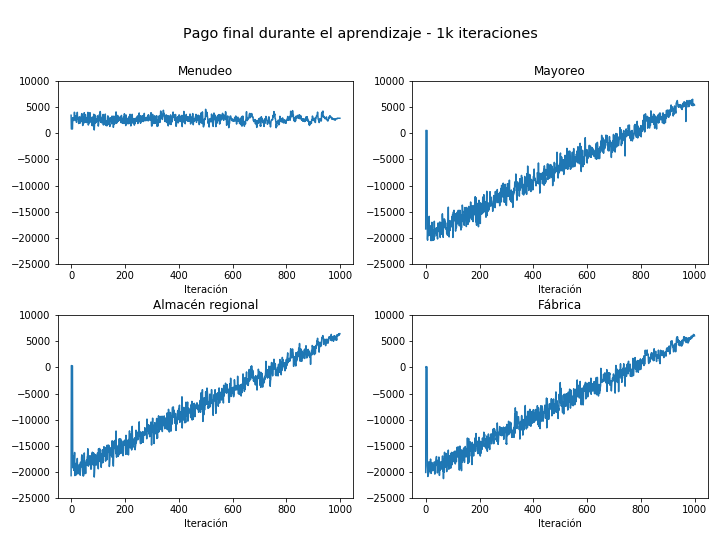
\includegraphics[width=1\linewidth]{tesis_tex/figs/policyiteration_payouts_1000.png}
     \caption{Evoluci\'on de recompensas con 1k iteraciones}\label{politer_payouts_1000}
   \end{minipage}\hfill
   \begin{minipage}{0.48\textwidth}
     \centering
     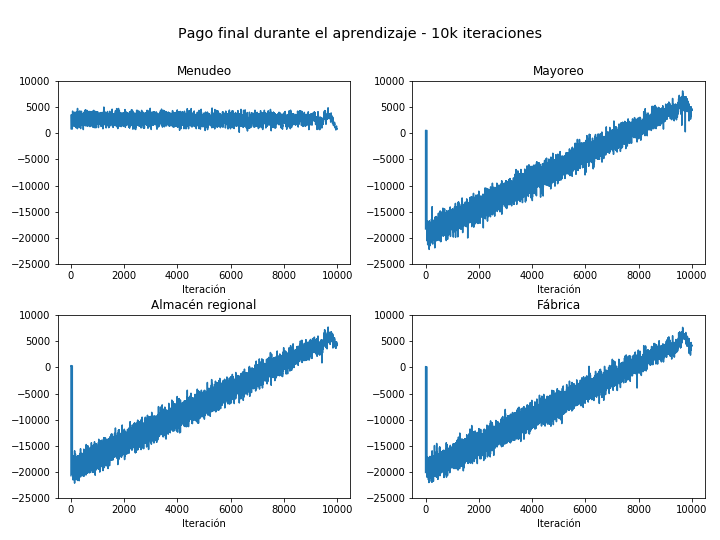
\includegraphics[width=1\linewidth]{tesis_tex/figs/policyiteration_payouts_10000.png}
     \caption{10k iteraciones}\label{politer_payouts_10000}
   \end{minipage}
\end{figure}

\begin{figure}[!htb]
   \begin{minipage}{0.48\textwidth}
     \centering
     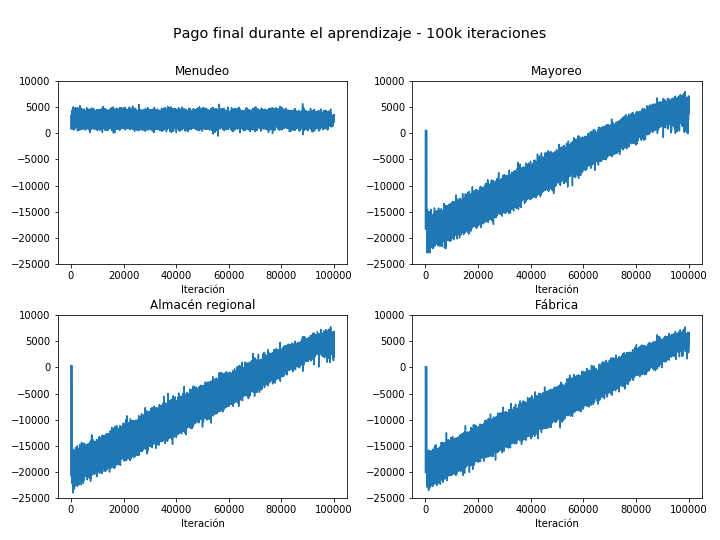
\includegraphics[width=1\linewidth]{tesis_tex/figs/policyiteration_payouts_100000.png}
     \caption{100k iteraciones}\label{politer_payouts_100000}
   \end{minipage}\hfill
   \begin{minipage}{0.48\textwidth}
     \centering
     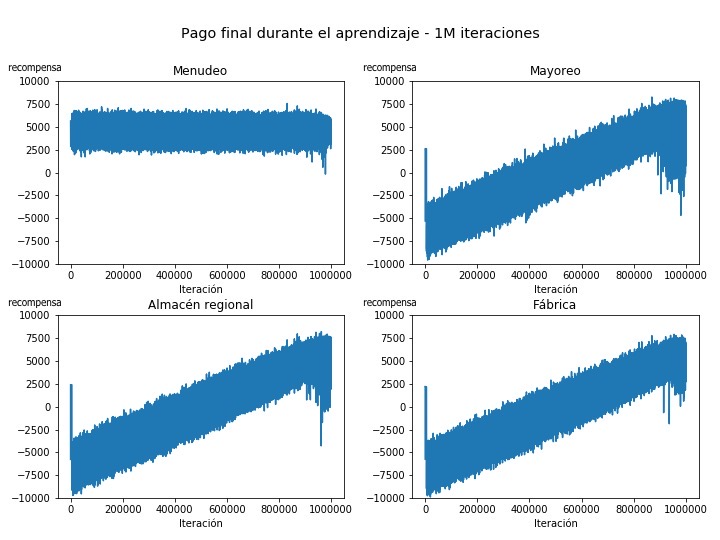
\includegraphics[width=1\linewidth]{tesis_tex/figs/policyiteration_payouts_1000000.png}
     \caption{1M iteraciones}\label{politer_payouts_1000000}
   \end{minipage}
\end{figure}

Es esperado observar  que todos los agentes presentan una tendencia positiva al encontrar mejores \textit{policies} en cada iteraci\'on del algoritmo. Sin embargo, es interesante notar que la funci\'on de valor del agente Menudeo empieza (despu\'es de un periodo de pre-calentamiento de $0.5\%$ del total de iteraciones) en un punto mucho m\'as cercano al \'optimo que los otros agentes. Esto puede explicarse porque, dada la configuraci\'on del mundo, el agente Menudeo tiene informaci\'on directa de la demanda del consumidor, y por lo tanto puede ajustar su pol\'itica mucho m\'as r\'apidamente.\\

El algoritmo converge de manera relativamente r\'apida: en las figuras  \ref{politer_payouts_1000} a \ref{politer_payouts_1000000} se puede observar que, con diferente n\'umero de iteraciones, el comportamiento del crecimiento de la funci\'on de valor (inferida de la pol\'itica \'optima en la iteraci\'on $i$) es similar. Asimismo, en las figuras \ref{politer_policies_1000} a \ref{politer_policies_1000000} se puede observar una comparaci\'on de las pol\'iticas obtenidas con los mismos umbrales de iteraciones: la forma es extremadamente parecida sin importar la cantidad de iteraciones. Este fen\'omeno nos indica que no es necesario un n\'umero alto de iteraciones, pues se encuentra el valor m\'aximo y la forma correcta de la pol\'itica \'optima solamente con solamente $10,000$ iteraciones. Con las condiciones de hardware y software especificadas en secciones anteriores, este proceso tarda un poco menos de 5 minutos.\\

Otra manera de analizar la r\'apida convergencia al \'optimo del algoritmo es comparando las recompensas finales (asociadas a la estrategia \'optima encontrada) para cada agente, con diferente n\'umero de iteraciones. En la figura \ref{money_over_time} se puede observar que, despu\'es de interaciones, el resultado final es sumamente estable.\\

\begin{figure}[H]
\caption{Comparaci\'on de recompensa final con diferente total de iteraciones}
\label{money_over_time}
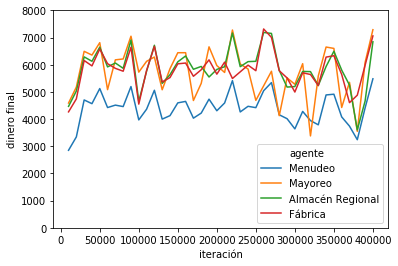
\includegraphics[width=10cm]{tesis_tex/figs/evaluating_interations_money.png}
\centering
\end{figure}

Las pol\'iticas aprendidas tienen el comportamiento esperado: todos los agentes compran cantidades altas durante ambos picos de producci\'on que se presentan alrededor de la mitad del a\~no para abastecerse lo m\'as posible para las ventas del resto del a\~no. Es importante recordar que estas pol\'iticas \'optimas dependen de la selecci\'on de par\'ametros del mundo (precios, costos, etc.) en gran medida, as\'i como los metapar\'ametros (tiempo de calentamiento, $\epsilon$, etc.) y esto implica que es necesario realizar un entrenamiento nuevo en caso de que estos cambien, o si de un a\~no a otro los agentes tienen, por ejemplo, diferentes inventarios iniciales. Este problema puede ser resuelto entrenando un modelo como \textit{Q-learning}, opci\'on que se explorar\'a levemente m\'as adelante en esta secci\'on.\\

\begin{figure}[!htb]
   \begin{minipage}{0.48\textwidth}
     \centering
     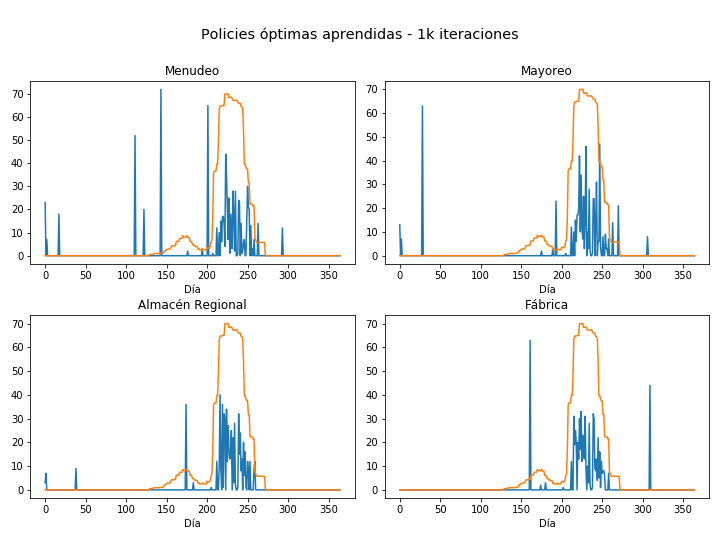
\includegraphics[width=1\linewidth]{tesis_tex/figs/policyiteration_policies_1000.png}
     \caption{Evoluci\'on de recompensas con 1k iteraciones}\label{politer_policies_1000}
   \end{minipage}\hfill
   \begin{minipage}{0.48\textwidth}
     \centering
     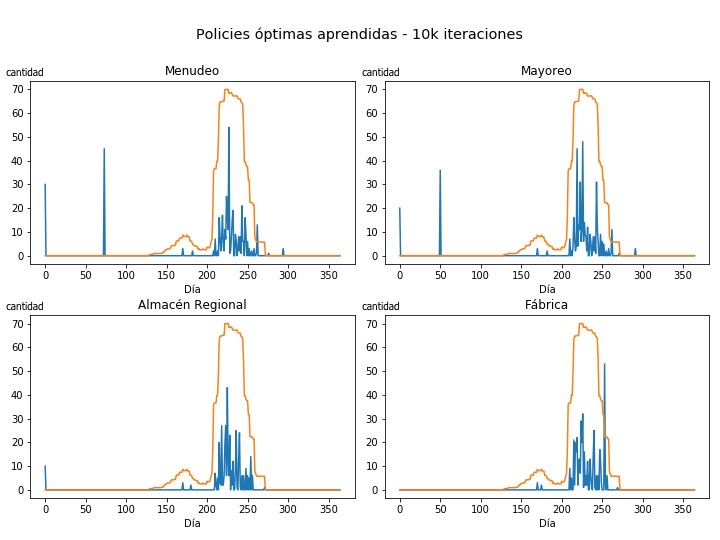
\includegraphics[width=1\linewidth]{tesis_tex/figs/policyiteration_policies_10000.png}
     \caption{10k iteraciones}\label{politer_policies_10000}
   \end{minipage}
\end{figure}

\begin{figure}[!htb]
   \begin{minipage}{0.48\textwidth}
     \centering
     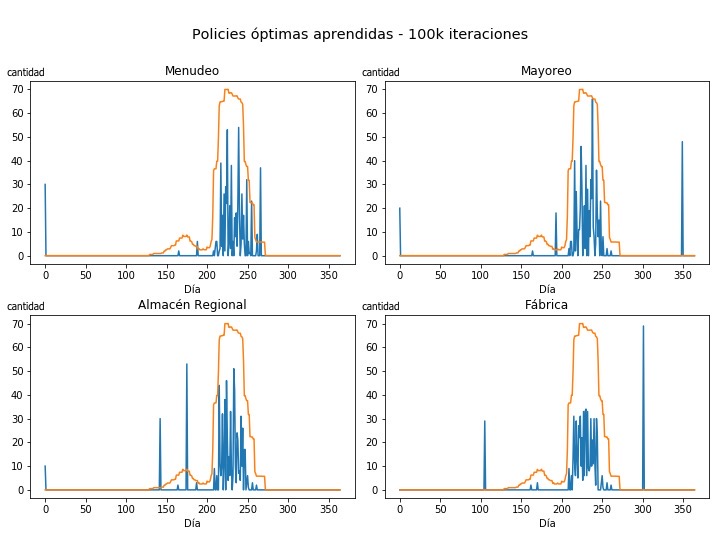
\includegraphics[width=1\linewidth]{tesis_tex/figs/policyiteration_policies_100000.png}
     \caption{100k iteraciones}\label{politer_policies_100000}
   \end{minipage}\hfill
   \begin{minipage}{0.48\textwidth}
     \centering
     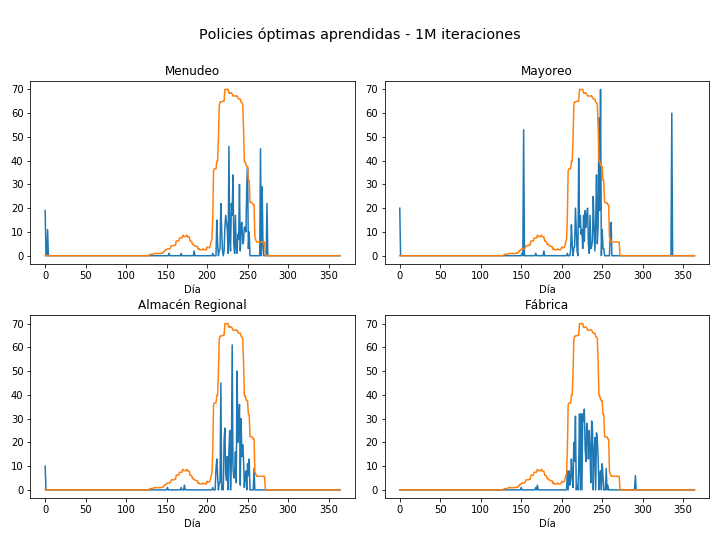
\includegraphics[width=1\linewidth]{tesis_tex/figs/policyiteration_policies_1000000.png}
     \caption{1M iteraciones}\label{politer_policies_1000000}
   \end{minipage}
\end{figure}

Durante el an\'alisis de las pol\'iticas y sus resultados, sali\'o a la luz un fen\'omeno no esperado: la penalizaci\'on por \'ordenes no cumplidas afecta de manera desequilibrada a los agentes.\\

Se ha hablado ya de las estrategias \'optimas obtenidas por el algoritmo de \textit{policy iteration}, sin embargo es de suma importancia comparar el potencial beneficio que podr\'ian tener los agentes tomando como l\'inea base una estrategia cre\'ible pero poco optimizada, en este caso definida como una estrategia b\'asica: cada agente calcula el promedio de peticiones del agente inferior durante los \'ultimos 5 d\'ias, y fija ese n\'umero como su demanda al agente superior. Por otro lado, la estrategia \'optima es el resultado del algoritmo \textit{policy iteration}. Una estrategia intermedia muestra solo un agente tomando las decisiones \'optimas, con los otros tres tomando los promedios.\\

Para este an\'alisis, se cre\'o un \'indice que se puede interpretar como la ganancia en porcentaje con respecto a la estrategia base, es decir, un valor del \'indice de $0.5\%$ significa que esa estrategia report\'o $50\%$ m\'as dinero al final de ese a\~no para ese agente que si hubiera tomado la estrategia de los promedios. Cualquier valor positivo del \'indice, entonces, implica un desempe\~no mejor que la l\'inea base, un valor negativo significa un desempe\~no peor.\\

Tambi\'en es relevante explorar si la estrategia \'optima es preferible en cualquier escenario respecto a los par\'ametros del mundo (inventarios iniciales, precios de compra/venta, costo de almacenamiento, entre otros). Para analizar este aspecto tambi'en, en cada nueva iteraci\'on se reinicializan todos los valores de tales par\'ametros de manera casi aleatoria; con restricciones de valores no-negativos para todos, y adicionalmente para los m\'argenes de los agentes. As\'i, el an\'alisis abarca una gran cantidad de casos y demuestra flexibilidad ante condiciones iniciales.\\

En la figura \ref{ev_policies_dumb} se puede ver una comparaci\'on del desempe\~no de todos los agentes con respecto a la l\'inea base elegida. Se muestra la l\'inea base, o la estrategia \textit{nadie \'optima} como una l\'inea azul punteada. Las dos curvas de comparaci\'on son: una combinaci\'on de estrategias en las que solamente el agente indicado toma y actualiza sus decisiones con el algoritmo de aprendizaje \textit{un agente \'optimo} y una combinaci\'on en la que todos los agentes aprenden con el algoritmo. Para esta figura se hicieron $250$ realizaciones del algoritmo con $1000$ etapas de aprendizaje, inicializando todos los par\'ametros del mundo de manera aleatoria cada vez, con restricciones m\'inimas relacionadas a los rangos de cada variable (por ejemplo, asegurar m\'argenes e inventarios no negativos)\\

En general, las distribuciones de índices relacionados a todos los agentes usando las estrategias \'optimas (obtenidas del algoritmo de aprendizaje) se encuentran a la derecha de las distribuciones de un solo agente aprendiendo. Esto es el comportamiento esperado, pues uno de los principales castigos para todos los agentes es el costo por orden no cumplida, y si no aprenden que deben tener suficiente inventario para cubrir esas \'ordenes, siempre cargar\'an con ese tipo de costos. Queda claro que es preferible para todos los agentes en conjunto trabajar de manera \'optima (con aprendizaje) al mismo tiempo, sin importar los par\'ametros iniciales de costos, inventarios o m\'argenes.\\

Sin embargo, es importante notar que las distribuciones de \'indices cuando solamente un agente utiliza la estrategia de aprendizaje se encuentran constantemente a la derecha de la l\'inea base. Esto quiere decir que siempre es preferible utilizar la estrategia de aprendizaje, sin importar la estrategia que el resto de los agentes escojan.\\

Una situaci\'on muy interesante se presenta en el escenario complementario al anterior: se ha establecido que es preferible usar la estrategia aprendida a pesar de que los otros agentes no hagan lo mismo, pero ¿qu\'e pasa con los agentes que no escogen la estrategia aprendida, cuando otro agente s\'i lo hace? El comportamiento esperado ser\'ia que la utilidad fuera mejor que si nadie estuviera aprendiendo, dado que al menos uno de los agentes estar\'ia optimizando su inventario. Esto se puede ver tambi\'en en la figura \ref{ev_policies_dumb}.\\

Por \'ultimo, podemos observar que las distribuciones de un solo agente tomando decisiones \'optimas son diferentes a pares: las de menudeo y f\'abrica son similares entre s\'i, al igual que las de mayoreo y almac\'en regional. Es notable que este comportamiento se presenta en los dos agentes que tienen una realidad diferente, ligada a agentes con estrategias estables y de donde provienen la demanda y oferta reales. El agente de menudeo siempre podr\'a vender todo su inventario lo m\'as pronto posible, dado que el comprador siempre tiene demanda positiva. Por otro lado, el agente de f\'abrica tambi\'en carga con presi\'on de los agentes inferiores de reducir sus costos de \'ordenes no cumplidas, as\'i que tambi\'en tiene asegurado vender su inventario pronto, mientras no compre cantidades innecesariamente altas. Los agentes de mayoreo y almac\'en regional no tienen ninguna de estas consideraciones. \\

En conclusi\'on, para cualquier agente es preferible usar la estrategia aprendida, sin importar lo que hagan los dem\'as agentes.


\begin{figure}[H]
\caption{Comparaci\'on de desempe\~no entre combinaciones de estrategias}
\label{ev_policies_dumb}
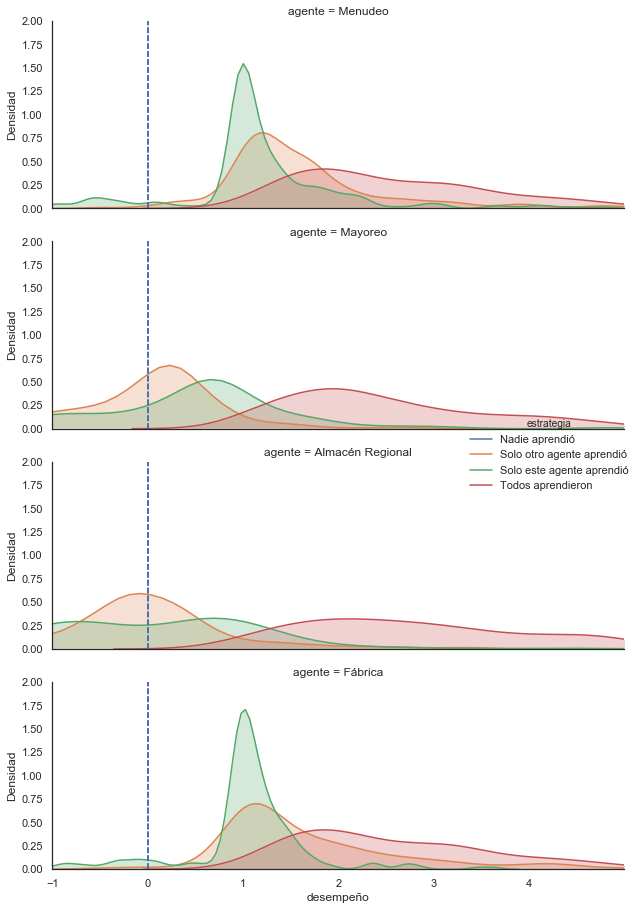
\includegraphics[width=9cm]{tesis_tex/figs/evaluating_policies_dumb_to_smart.png}
\centering
\end{figure}

\section{Q-Learning}

A diferencia de \textit{policy iteration}, este m\'etodo encuentra, para cada estado, la acci\'on que acercar\'a al agente lo m\'as posible a la meta. Por supuesto, la pol\'itica \'optima es equivalente con cualquiera de ambos m\'etodos, pero \textit{Q-learning} permite m\'as libertad respecto a empezar a jugar el juego a mitad de a\~no, arreglar malas decisiones tomadas por los agentes en periodos anteriores gracias a su adaptabilidad ante cambios estoc'asticos, etc.\\

Las ecuaciones que describen el aprendizaje de un agente son:

\begin{enumerate}
    \item La ecuaci\'on de utilidad (o recompensa) para cada agente $a$ en el d\'ia $d$:

$$
R(a, d) = r(a,d) + \gamma*r_{a, d+1} + ... + \gamma^{364}*r_{a,d+364}
$$

Donde la recompensa del agente \textit{a} en el d\'ia \textit{d} es la ganancia relacionada a sus respectivas transacciones, como se defini\'o al principio de este cap\'itulo. Es importante notar la importancia de tomar un periodo de un a\~no despu\'es del d\'ia $d$ sin importar en qu\'e d\'ia espec\'ifico se encuentre el agente: de esta manera, el agente aprender\'a si tiene que llegar al d\'ia $365$ con inventario en almacenes.

    \item La funci\'on Q para cada agente $a$ dado su estado, el d\'ia $d$ con cierto inventario $inv$:

$$
Q_{a}(inv_{d},compra_{d}) = r_{a, (d, inv, compra)} + \gamma * \max_{compras}{Q_{a}(inv_{d} + compra_{d}, compras_{d+1}}
$$

Para cada agente, su estado es un vector de longitud $2$: en el d\'ia $d$ es el inventario que tiene en el almac\'en, y las acciones que puede tomar en cada estado se representan como un vector de longitud $1$: son las diferentes cantidades que puede comprarle al agente superior.
\end{enumerate}

Adem\'as, se implement\'o este algoritmo en la modalidad \textit{greedy}, con $\epsilon$ empezando en $1.00$ y terminando en $0.05$.

